\documentclass[12pt]{article}
\usepackage[polish]{babel}
\usepackage[T1]{fontenc}

\usepackage{graphicx} % Required for inserting images
\graphicspath{ {rysunki/} }
\usepackage{fontspec}
\usepackage{pdfpages}
\usepackage{geometry}
\usepackage{setspace}
\usepackage{titlesec}
\usepackage{import}
\usepackage{indentfirst}
\usepackage{float}
\usepackage{caption}
\usepackage{amsmath}
\usepackage{amssymb}
\usepackage{tocloft}
\usepackage{multirow}
\usepackage{xltabular}
\usepackage[hidelinks]{hyperref}
\usepackage{xurl}
\emergencystretch=3em
\usepackage{csquotes}           
\usepackage[
    backend=biber,
    style=numeric,
    sorting=none,
    giveninits=true,
    url=true,
    doi=false,
    isbn=false,
    eprint=false
]{biblatex}
\setcounter{biburlnumpenalty}{7000}
\setcounter{biburlucpenalty}{8000}
\setcounter{biburllcpenalty}{9000}
\urlstyle{same}
\addbibresource{bibliografia.bib}

\onehalfspacing
 \geometry{
 a4paper,
 lmargin=35mm,
 rmargin=20mm,
 tmargin=25mm,
 bmargin=25mm,
 }
\setmainfont{Times New Roman}
\setlength\parindent{1cm}

\titleformat{\section}{\normalfont\Large\fontsize{16}{16}\bfseries}{\thesection.}{0.76cm}{}
\titlespacing*{\section}
{0pt}{24pt}{24pt}

\titleformat{\subsection}{\normalfont\Large\fontsize{14}{14}\bfseries}{\thesubsection.}{1.02cm}{}
\titlespacing*{\subsection}
{0pt}{12pt}{12pt}

\numberwithin{figure}{section}
\DeclareCaptionLabelSeparator{custom}{. }
\captionsetup[figure]{
    name=Rys.,
    labelsep=custom,
    font={footnotesize},
    justification=centering
}

\numberwithin{table}{section}
\DeclareCaptionLabelSeparator{custom}{. }
\captionsetup[table]{
    labelsep=custom,
    font={footnotesize},
    justification=centering
}

\setlength{\abovecaptionskip}{0pt}
\setlength{\belowcaptionskip}{10pt}

\renewcommand{\cftsecpresnum}{}
\renewcommand{\cftsecaftersnum}{.}
\renewcommand{\cftsubsecaftersnum}{.}

\begin{document}


\includepdf[pages=-]{strona-tytulowa.pdf}
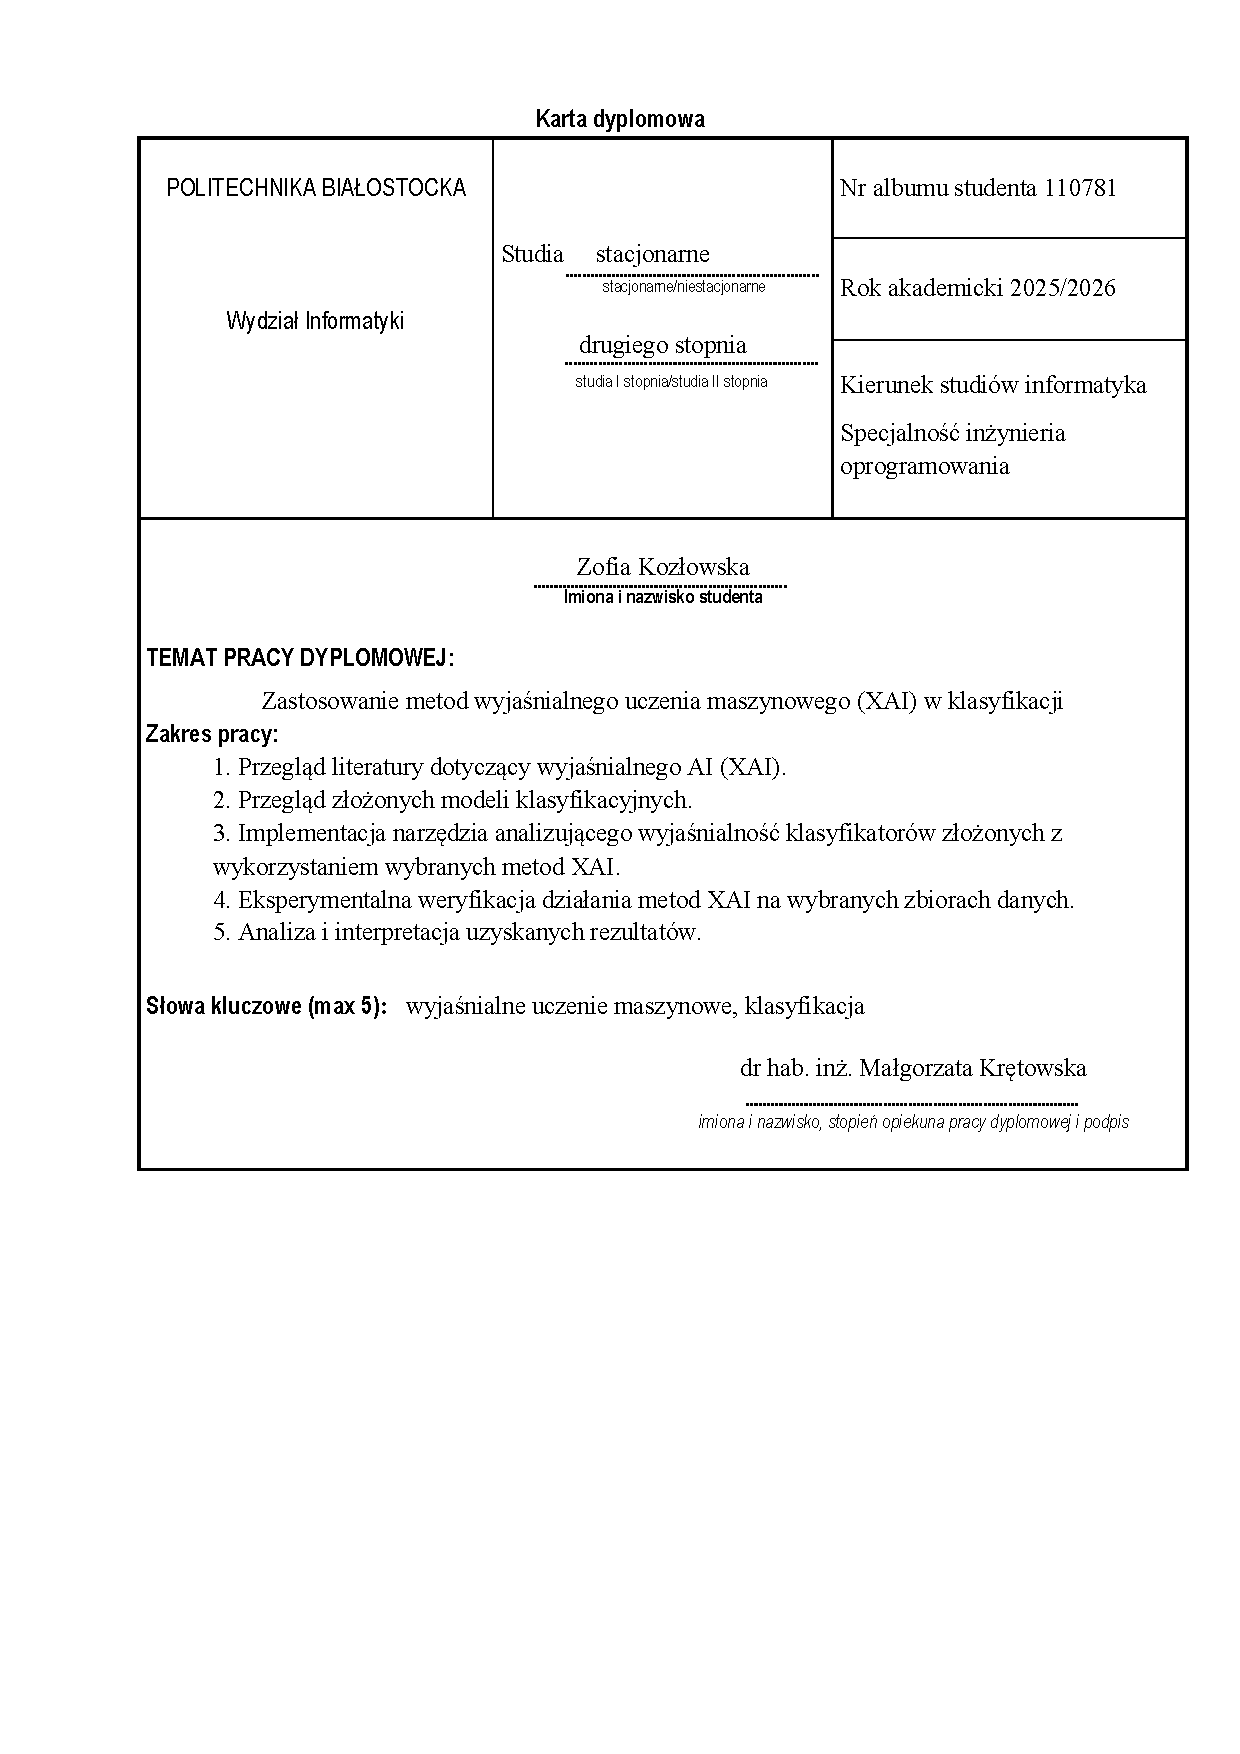
\includepdf[pages=-]{Karta Dyplomowa 2026-03-05.pdf}
\includepdf[pages=-]{streszczenie-ang.pdf}
\includepdf[pages=-]{Oswiadczenia-o-wykorzystaniu-narzedzi-GenAI.pdf}

\newpage
\tableofcontents
\thispagestyle{empty}

\newpage
\setcounter{page}{1}
\import{rozdzialy/}{wstep.tex}

\newpage
\import{rozdzialy/}{wprowadzenie_do_problemu.tex}

\newpage
\import{rozdzialy/}{problem_klasyfikacji.tex}

\newpage
\import{rozdzialy/}{metody_xai.tex}

\newpage
\import{rozdzialy/}{opis_implementacji.tex}

\newpage
\import{rozdzialy/}{eksperymenty.tex}

\newpage
\import{rozdzialy/}{podsumowanie.tex}

\newpage
\pagestyle{empty}
\cleardoublepage
\phantomsection
\printbibliography[heading=bibintoc,title={Literatura}]
\end{document}